\documentclass[12pt]{article}
\usepackage[margin=1in]{geometry} 
\usepackage{amsmath,amsthm,amssymb,amsfonts}
\usepackage{enumerate,listings,graphicx,epstopdf,siunitx}
\usepackage{color}
\graphicspath{~/Documents/school/fall16/stat586/hw3}

\sloppy
\definecolor{lightgray}{gray}{0.5}
 
\newcommand{\N}{\mathbb{N}}
\newcommand{\Z}{\mathbb{Z}}
\newcommand{\normD}[3]{\frac{1}{\sqrt{2\pi #1^2}}exp(\frac{-( #2 - #3)^2}{2 #1^2})} 
\newenvironment{problem}[2][Problem]{\begin{trivlist}
\item[\hskip \labelsep {\bfseries #1}\hskip \labelsep {\bfseries #2.}]
  \vspace{1 cm}
}{\end{trivlist}}

\begin{document}
\title{Homework Set 4}
\author{Taylor Bodin}
\maketitle

\section*{Problem 3.35}
\subsection*{a.}
\begin{align*}
  f_{X|X>0} &= \frac{P(X \leq x, 0<X<\infty)}{P(0<X<\infty)} \\
  &= \begin{cases} 
        \frac{f_X(x)}{P(0<x)}, & 0 < x < \infty \\
        0, & otherwise 
     \end{cases} \\
  &= \begin{cases} 
        \frac{1}{2\sqrt{2\pi\sigma^2}}exp(\frac{-x^2}{2\sigma^2}), & 0 < x < \infty \\
        0, & otherwise 
      \end{cases}
\end{align*}

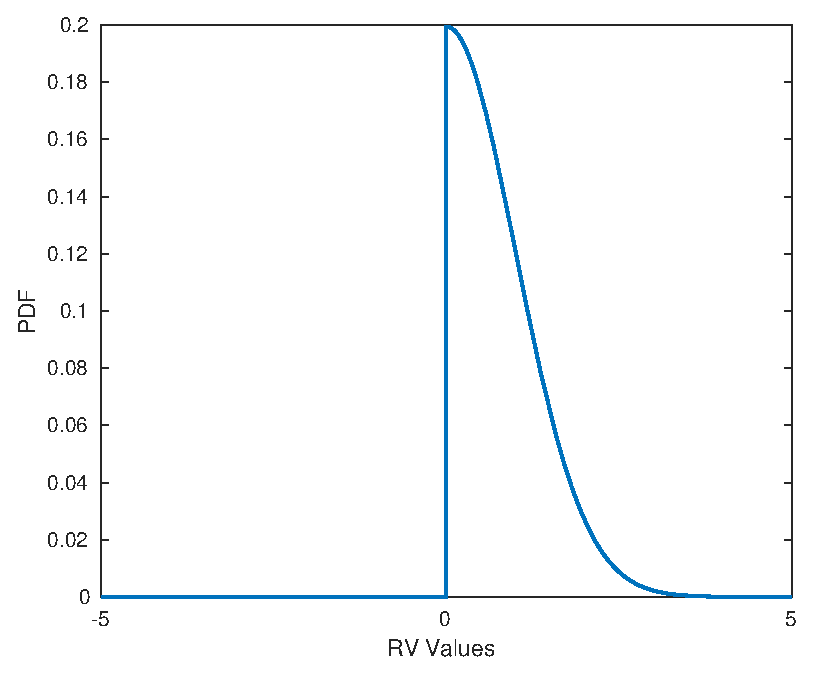
\includegraphics [width=4in]{fig_3_35_a.eps}
\subsection*{b.}
\begin{align*}
  f_{X||X|>3} &= \frac{P(X \leq x, -3<X<3)}{P(-3<X<3)} \\
  &= \begin{cases} 
    \frac{f_X(x)}{P(-3<x<3)}, & -3 < x < 3 \\
    0, & otherwise 
  \end{cases} \\
  &= \begin{cases} 
    \frac{\frac{1}{2\sqrt{2\pi\sigma^2}}exp(\frac{-x^2}{2\sigma^2})}
    {Q(\frac{-3}{\sigma}) - Q(\frac{3}{\sigma})}, & 0 < x < \infty \\
    0, & otherwise 
  \end{cases} \\
  &= \begin{cases} 
    \frac{1}{2\sqrt{2\pi\sigma^2}}exp(\frac{-x^2}{2\sigma^2})
    \frac{1}{1 - 2Q(\frac{3}{\sigma})}, & 0 < x < \infty \\
    0, & otherwise 
  \end{cases}
\end{align*}

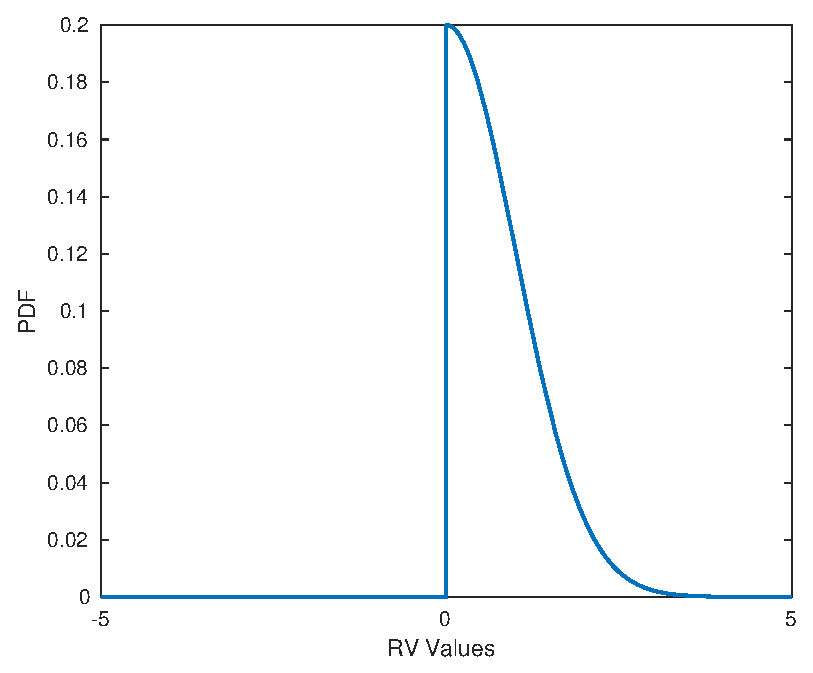
\includegraphics [width=4in]{fig_3_35_b.eps}
\subsection*{c.}
\begin{align*}
  f_{X||X|<3} &= \frac{P(X \leq x, -3>X \cup  X>3)}{P(-3>X \cup  X>3)} \\
  &= \begin{cases} 
    \frac{f_X(x)}{P(-3>X \cup  X>3)}, &  -3>X \textrm{ or } X>3\\
    0, & otherwise 
  \end{cases} \\
  &= \begin{cases} 
    \frac{\frac{1}{2\sqrt{2\pi\sigma^2}}exp(\frac{-x^2}{2\sigma^2})}
    {1- Q(\frac{-3}{\sigma}) + Q(\frac{3}{\sigma})}, & -3>X \textrm{ or } X>3 \\
    0, & otherwise 
  \end{cases} \\
  &= \begin{cases} 
    \frac{1}{2\sqrt{2\pi\sigma^2}}exp(\frac{-x^2}{2\sigma^2})
    \frac{1}{2Q(\frac{3}{\sigma})}, &  -3>X \textrm{ or } X>3 \\
    0, & otherwise 
  \end{cases}
\end{align*}

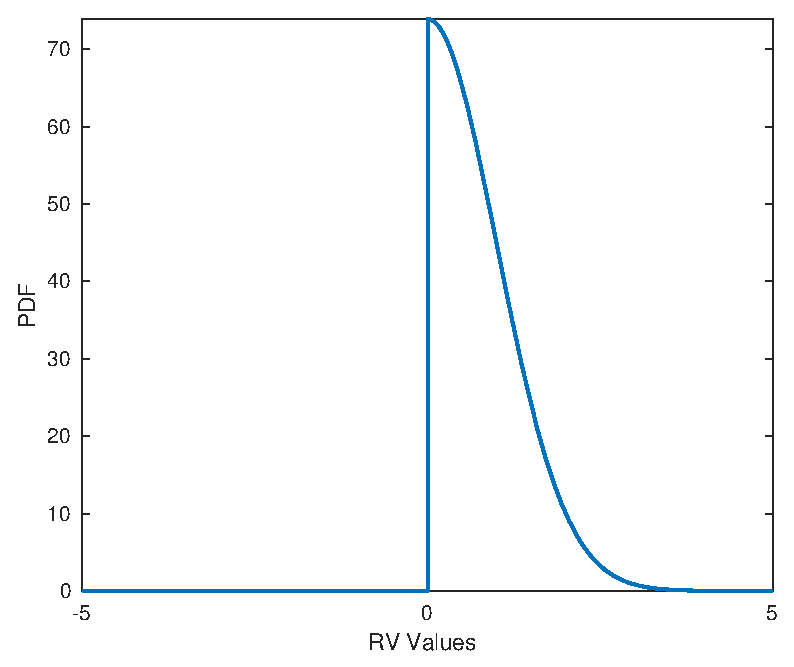
\includegraphics [width=4in]{fig_3_35_c.eps}

\section*{Problem 3.37}
\subsection*{a.}
\subsubsection*{Find an expresion for $P_{m=0|X=x}$}
\begin{align*}
  P_{m=0|X=x} &= \frac{f_{x|m=0}P(m=0)}{f_{x|m=0}P(m=0)+f_{x|m=1}P(m=1)} \\
  &= \frac{.5\normD{\sigma}{x}{0}}{.5\normD{\sigma}{x}{0}+.5\normD{\sigma}{x}{1}} \\
  &= \frac{exp(\frac{-x^2}{2\sigma^2})}
    {exp(\frac{-x^2}{2\sigma^2})+exp(\frac{-(x-1)^2}{2\sigma^2})} \\
  &= \frac{\sqrt{e}}{\sqrt{e}+e^x} 
\end{align*}
\subsubsection*{Find an expresion for $P_{m=1|X=x}$}
\begin{align*}
  P_{m=1|X=x} &= \frac{f_{x|m=1}P(m=1)}{f_{x|m=0}P(m=0)+f_{x|m=1}P(m=1)} \\
  &= \frac{.5\normD{\sigma}{x}{1}}{.5\normD{\sigma}{x}{0}+.5\normD{\sigma}{x}{1}} \\
  &= \frac{exp(\frac{-(x-1)^2}{2\sigma^2})}
    {exp(\frac{-x^2}{2\sigma^2})+exp(\frac{-(x-1)^2}{2\sigma^2})} \\
  &= \frac{e^x}{\sqrt{e}+e^x} 
\end{align*}
\subsubsection*{Find X such that $P \geq .9$ for each case and E otherwise}
\[
\begin{cases}
  1, & x > 2.697 \\
  E, & -1.698 < x < 2.697 \\
  0, & x < -1.697 
\end{cases}
\]
\subsection*{b.}
\begin{align*}
  P(E) &= P(X<2.697|m=1)P(m=1)+P(X>-1.697|m=0)P(m=0) \\
  &= (1 - Q(\frac{2.697-1}{1})).5 + Q(\frac{-1.697}{1}).5 \\
  &= .9552(.5) + .9552(.5) = .9552
\end{align*}
\subsection*{c.}
\begin{align*}
  P(\textrm{error}) &= P(X>2.697|m=0)P(m=0)+P(X<-1.697|m=1)P(m=1) \\
  &= Q(2.697)(.5) + 1 - Q(-2.697)(.5) \\
  &= Q(2.697) = .0035
\end{align*}

\section*{Problem 3.39}
\subsection*{a.}
\begin{align*}
  f_{V|V>1} &= \begin{cases} 
     \frac{f_V(v)}{P(1<v)}, & 1 < v < 2 \\
        0, & otherwise 
     \end{cases} \\
    &= \begin{cases} 
      \frac{.5}{.5}, & 1 < v < 2 \\
        0, & otherwise 
      \end{cases} \\
    &= \begin{cases} 
      \frac{1}{4}, & 1 < v < 2 \\
        0, & otherwise 
      \end{cases}
\end{align*}
\subsection*{b.}
\begin{align*}
  f_{V|} &= \begin{cases} 
    \frac{f_V(v)}{P(\frac{1}{2}<v<\frac{3}{2})}, & \frac{1}{2}<v<\frac{3}{2} \\
        0, & otherwise 
     \end{cases} \\
    &= \begin{cases} 
      \frac{.5}{.5}, & \frac{1}{2}<v<\frac{3}{2} \\
        0, & otherwise 
      \end{cases} \\
    &= \begin{cases} 
      \frac{1}{4}, & \frac{1}{2}<v<\frac{3}{2} \\
        0, & otherwise 
      \end{cases}
\end{align*}
\subsection*{c.}
\begin{align*}
  F_{V|\frac{1}{2}<V<\frac{3}{2}} &= 
  \begin{cases} 
    0, & V<\frac{1}{2} \\
    \frac{f_V(v) - f_V(.5)}{f_V(1.5) - f_V(.5)}, & \frac{1}{2}<v<\frac{3}{2} \\
    1, & V>\frac{3}{2}
  \end{cases} \\
 &= \begin{cases} 
    0, & V<\frac{1}{2} \\
    v-\frac{1}{2}, & \frac{1}{2}<v<\frac{3}{2} \\
    1, & V>\frac{3}{2}
  \end{cases}  
\end{align*}

\section*{Problem 3.41}
\subsection*{Setup}
$R_{1 unit} = \lambda_n = \frac{1}{100} \textrm{days}^{-1}$ \\
$R_{system} = \sum_{n=1}^{10} R_{1_unit} = (10)\frac{1}{100} = \frac{1}{10} \textrm{days}^{-1}$

\subsection*{a.}
\[
  P(L_{system} > 100) = exp(-(\frac{1}{10} \textrm{days}^{-1})(10 \textrm{days})) = e^{-1} = .3679
\]
\subsection*{b.}
\[
  P(L_{unit} > 100) = exp(-(\frac{1}{100} \textrm{days}^{-1})(10 \textrm{days})) = e^{-1} = .9048
\]
\section*{Problem 3.43}
\subsection*{c.}
$R_{1 unit} = \lambda_n = \frac{1}{100} \textrm{days}^{-1}$ \\
$R_{system} = \sum_{n=1}^{10} R_{1_unit} = (10)\frac{1}{100} = \frac{1}{10} \textrm{days}^{-1}$

\subsection*{a.}
\begin{align*}
  P(S|x=200) &= \frac{P(S|x=200)P(S)}{P(S|x=200)P(S)+P(L|x=200)P(L)} \\
  &= \frac{.75(\frac{1}{100}exp(\frac{-200}{100}))}{.75(\frac{1}{100}exp(\frac{-200}{100})
    .25(\frac{1}{1000}exp(\frac{-200}{1000})} \\
  &= .8322
\end{align*}

\subsection*{b.}
\begin{align*}
  P(L|x=200) &= \frac{P(L|x=200)P(L)}{P(S|x=200)P(S)+P(L|x=200)P(L)} \\
  &= \frac{.25(\frac{1}{1000}exp(\frac{-200}{1000}))}{.75(\frac{1}{100}exp(\frac{-200}{100})
    .25(\frac{1}{1000}exp(\frac{-200}{1000})} \\
  &= .1678
\end{align*}

\section*{Problem 3.45}
\subsection*{a.}
\begin{align*}
  SSE &= \sum_{n=1}^k \left( F_n - (1 - exp(\frac{-x_n^2}{2\sigma^2}))^2 \right) \\
  \frac{d}{d\sigma^2}SSE &= \frac{d}{d\sigma^2}\sum_{n=1}^k \left( F_n - (1 - exp(\frac{-x_n^2}{2\sigma^2}))^2 \right) \\
  0 &= \frac{2}{\sigma^3}\sum_{n=1}^k \left( F_n - (1 - exp(\frac{-x_n^2}{2\sigma^2}))\right)exp(\frac{-2x_n^2}{2\sigma^2})x_n^2
\end{align*}

\subsection*{b.}
\begin{align*}
  SSE &= \sum_{n=1}^k \left( log(1-Fn) + \frac{-x_n^2}{2\sigma^2} \right)^2 \\
  \frac{d}{d\sigma^2}SSE &= \frac{d}{d\sigma^2} \sum_{n=1}^k \left( log(1-Fn) + \frac{-x_n^2}{2\sigma^2} \right)^2 \\
  0 &= \sum_{n=1}^k 2(log(1-F_n) + \frac{x_n^2}{2\sigma^2}(\frac{-x_n^2}{2\sigma^4}) \\
  0 &= \sum_{n=1}^k 2(x_n^2 log(1-F_n) + \frac{x_n^4}{2\sigma^2}) \\
  \frac{1}{\sigma^2} \sum_{n=1}^k x_n^4 &= \sum_{n=1}^k x_n^2 log(1-F_n) \\
  \sigma^2 &= -\frac{\sum_{n=1}^k x_n^4}{\sum_{n=1}^k x_n^2 log(1-F_n)}
\end{align*}
\section*{Problem 4.1}
\subsection*{a.}
\begin{align*}
  \mu_\omega &= \int_{-\infty}^{\infty} \omega f_\omega(\omega) d_\omega \\
   &= \int_{a}^{b} \frac{\omega}{b-a} d_\omega \\
   &= \frac{\omega^2}{2(b-a)} \big|_a^b \\
   &= \frac{b^2}{2(b-a)}-\frac{a^2}{2(b-a)} \\
   &= \frac{b^2}{2(b-a)}-\frac{a^2}{2(b-a)} \\
   &= \frac{b^2-a^2}{2(b-a)}
\end{align*}
\subsection*{b.}
\begin{align*}
  \mu_x &= \int_{-\infty}^{\infty} x f_x(x) d_x \\
   &= \int_{0}^{1} 3x^3 d_x \\
   &= x^4 \big|_0^1 \\
   &= 1-0 = 1 
 \end{align*}
\subsection*{c.}
\begin{align*}
  \mu_y &= \int_{-\infty}^{\infty} y f_y(y) d_y \\
   &= 6\int_{0}^{1} y^2(1-y) d_y \\
   &= 6(\frac{y^3}{3} - \frac{y^4}{4}) \big|_0^1 \\
   &= 6(\frac{1}{3} - \frac{1}{4}) \\
   &= 6(\frac{1}{12}) \\
   &= \frac{1}{2} 
 \end{align*}
\subsection*{d.}
\begin{align*}
  \mu_z &= \int_{-\infty}^{\infty} z f_z(z) d_z \\
  &= 6\int_{0}^{\infty} \frac{2z}{\pi(1+z^2)} d_z & & \textrm{Let } u = z^2+1, \ du = 2z \\
  &= \frac{ln(z^2+1)}{\pi} \big|_0^\infty \\
  &= \infty \\
 \end{align*}
\section*{Problem 4.3}
\subsection*{a.}
\begin{align*}
  E[w] &= \int_0^\infty (1-F_w(w))dw & & \textrm{with non-negative support} \\
  E[w] &= \int_0^\infty (1-\frac{w}{10})dw \\
  &= w - \frac{w}{20}\big|_0^{10} \\
  &= 10 - \frac{100}{20} = \frac{1}{2}
\end{align*}

\subsection*{b.}
\begin{align*}
  E[x] &= \int_0^\infty (1-F_x(x))dx & & \textrm{with non-negative support} \\
  E[x] &= \int_0^\infty 1-[1-exp(-2x)]dx \\
  &= w - \frac{-exp(-2x)}{2}\big|_0^\infty \\
  &= 0 - (\frac{-1}{2}) = \frac{1}{2}
\end{align*}

\subsection*{c.}
\begin{align*}
  E[y] &= \int_0^\infty (1-F_y(y))dy & & \textrm{with non-negative support} \\
  E[y] &= \int_0^2 1-\frac{y^2}{4} dy \\
  &= y - \frac{y^3}{12}\big|_0^2 \\
  &= 2 - (\frac{-8}{12}) = \frac{2}{3}
\end{align*}

\subsection*{d.}
\begin{align*}
  E[z] &= \int_0^\infty (1-F_z(z))dz & & \textrm{with non-negative support} \\
  E[z] &= \int_0^\infty 1-[1-exp(-z^2)]dz \\
  &= \frac{\sqrt{\pi}}{2}erf(z)\big|_0^\infty \\
  &= \frac{\sqrt{\pi}}{2}[1-0] = \frac{\sqrt{\pi}}{2}
\end{align*}

\section*{Problem 4.5}
\begin{align*}
  E[x] &= \int_0^\infty (1-F_X(x))dx \\
  &= \int_0^\infty \int_x^\infty f_X(y)dydx \\
  &= \int_0^\infty f_X(y) \int_0^y dx \\
  &= \int_0^\infty yf_X(y)
\end{align*}  
\section*{Problem 4.7}
\begin{align*}
  P_{avg} &= E[P] = E[X^2R] \\
&= \left[E[RX^2] + V[RX]\right] \\
&= R\left[E[X^2] + V[X]\right] \\
&= \SI{75}{\ohm}\left[0 + \SI{15}{\milli\ampere}\right] \\
&= \SI{75}{\ohm}(\SI{15}{\milli\ampere})^2 \\
&= \SI{16.875}{\milli\watt} \\
\end{align*}
\section*{Problem 4.9}
\begin{align*}
  E[|x|] &= \int_{-\infty}^{\infty} |x|\normD{\sigma}{x}{\mu} dx,
    & & \textrm{Let } x = \mu + \sigma t \\
  &= \int_{-\infty}^{\infty} |\mu+\sigma t| \frac{1}{\sqrt{2\pi\sigma^2}}
    exp(\frac{-t^2}{2})dx \\
    &= \int_{-\infty}^{\frac{-\mu}{\sigma}}(\mu+\sigma t)\frac{1}{\sqrt{2\pi\sigma^2}}exp(\frac{-t}{2})dt \\
    &+ \int_{\frac{-\mu}{\sigma}}^\infty{\sigma}(\mu+\sigma t)\frac{1}{\sqrt{2\pi\sigma^2}}exp(\frac{-t}{2})dt \\
    &=\frac{\sigma}{\sqrt{2\pi}}\left[\int_{\frac{-\mu}{\sigma}}^\infty t \ exp(\frac{-t^2}{2}) -
    \int_{\frac{-\mu}{\sigma}}^\infty t \ exp(\frac{-t^2}{2})\right] \\
    &+ \mu\left[\int_{\frac{-\mu}{\sigma}}^\infty \frac{1}{\sqrt{2\pi}}exp(\frac{-t^2}{2})  -
    \int_{\frac{-\mu}{\sigma}}^\infty \frac{1}{\sqrt{2\pi}}exp(\frac{-t^2}{2}) \right] \\
    &=\frac{\sigma}{\sqrt{2\pi}}\left[-exp(\frac{-t^2}{2})\big|_{\frac{-\mu}{\sigma}}^\infty +
    exp(\frac{-t^2}{2})\big|_{-\infty}{\frac{-\mu}{\sigma}}\right] \\
    &+ \mu\left[Q(\frac{-\mu}{\sigma}) -[1-Q(\frac{-\mu}{\sigma})]\right]  \\
    &= \frac{\sigma}{\sqrt{2\pi}}\left[ 0 + exp(\frac{-\frac{-\mu}{\sigma}}{2}) + exp(\frac{-\frac{-\mu}{\sigma}}{2}) - 0 \right]
    + 2\mu Q(\frac{-\mu}{\sigma})-\mu \\
    &= \frac{\sigma}{\sqrt{2\pi}} 2exp\left(-\frac{-\mu}{2\sigma}\right) + 2\mu Q\left(\frac{-\mu}{\sigma}\right)-\mu
\end{align*}
\section*{Problem 4.93}
\subsection*{a.}
If $X \sim unif[0,100]$ then $X$ is also distributed uniformly on the subinterval $[x,x+1]$ where $x \in [0,100]\cap \Z$
Therefore, Z's support is on $[-.5,.5]$ which is the furthest distance Y can be from X for any rounding error. Then Z's
PDF is also uniform and given by: \\
\[ \begin{cases} 
        1, & -.5 < z < .5 \\
        0, & otherwise 
    \end{cases} 
\] \\

It's also easy to determine the mean squared value using known values for a uniform distribution. 
\begin{align*}
  E[Z^2] &= E[Z]^2 + V[Z] \\
  &= .5[-.5 + .5] + \frac{1}{12}[.5-(-.5)] \\
  &= \frac{1}{12}
\end{align*}

\subsection*{b.}

\begin{verbatim}
close all; clear; clc;
\end{verbatim}


\subsubsection*{Create Z}

\begin{verbatim}
X = rand(200000,1);
Y = round(X);
Z = X-Y;
\end{verbatim}


\subsection*{Plot}

\begin{verbatim}
figure(1);
xlabel('Z values')
ylabel('Probability')
grid on
hold on
histogram(Z,200,'Normalization','pdf');
legend('Simulated Z');
\end{verbatim}

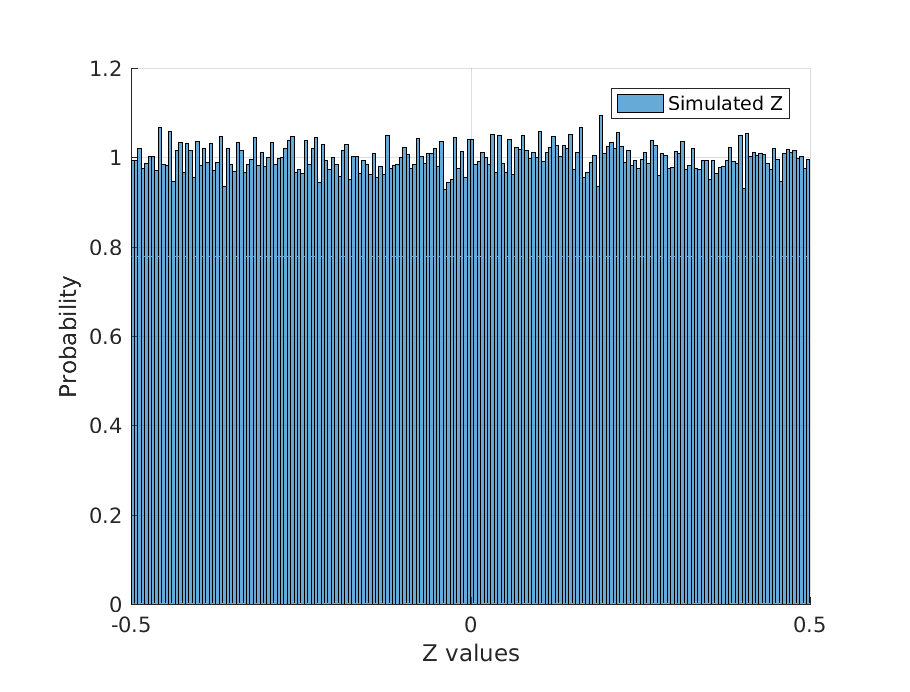
\includegraphics [width=4in]{problem_4_93_01.eps}
\section*{Problem 4.95}
\subsection*{Setup}
\begin{verbatim}
close all; clear; clc;
\end{verbatim}


\subsection*{Simulate X}

\begin{verbatim}
mu = 20;
sigma = 4;
N = 200000;

X = sigma*randn(N,1)+mu;
\end{verbatim}


\subsection*{Sample Mean}
This one seems to give the best estimate of the true mean for this distribution
\begin{verbatim}
sm = mean(X);
disp(sm);
\end{verbatim}

        \color{lightgray} \begin{verbatim}   20.0045

\end{verbatim} \color{black}
    

\subsection*{Geometric Mean}

\begin{verbatim}
gm = geomean(X);
disp(gm);
\end{verbatim}

        \color{lightgray} \begin{verbatim}   19.5826

\end{verbatim} \color{black}
    

\subsection*{Harmonic Mean}

\begin{verbatim}
hm =  harmmean(X);
disp(hm);
\end{verbatim}

        \color{lightgray} \begin{verbatim}   19.1246

\end{verbatim} \color{black}
    

\subsection*{Quadratic Mean}

\begin{verbatim}
rms = rms(X);
disp(rms);
\end{verbatim}

        \color{lightgray} \begin{verbatim}   20.3989

\end{verbatim} \color{black}

\subsection*{Plot}

\begin{verbatim}
figure(1);
xlabel('X values')
ylabel('Count')
grid on
hold on
histogram(X,200);
legend('Simulated X');
\end{verbatim}

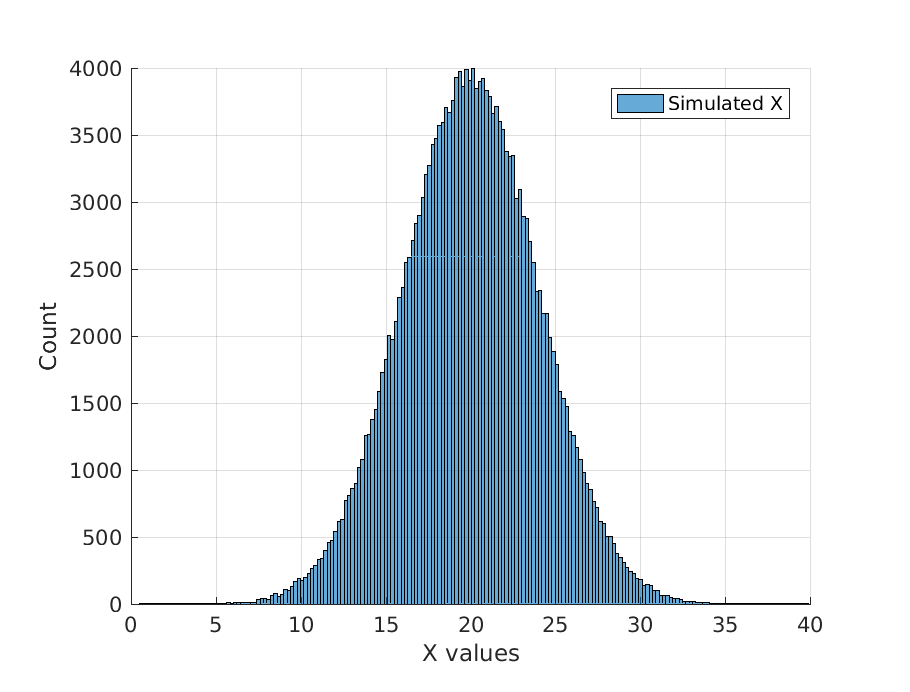
\includegraphics [width=4in]{problem_4_95_01.eps}
\section*{Problem 4.97}

\begin{verbatim}
function H = text_freq(input_file)
\end{verbatim}
\subsection*{IO functions}

\begin{verbatim}
text = fopen(input_file);
chars = fscanf(text, '%c');
\end{verbatim}
   
\subsection*{Massage the data}

\begin{verbatim}
letters = chars((chars>= 65) & (chars <= 122));
letters = lower(letters);
\end{verbatim}

\subsection*{Count the characters}

\begin{verbatim}
let_count = zeros(1,26);

for n = 1:26
let_count(n) = sum(letters == 96+n);
end
\end{verbatim}

\subsection*{Calculate the pmf}

\begin{verbatim}
pmf = let_count./length(letters);
\end{verbatim}

\subsection*{Calculate entropy}
Note: I borrowed the code for this section after reading a stack exchange on calculating entropy. The link is: \\
http://stackoverflow.com/questions/22074941/shannons-entropy-calculation

\begin{verbatim}
H = sum(-(pmf(pmf>0).*(log2(pmf(pmf>0)))));

return
\end{verbatim}
\subsection*{Problem 4.97 Test Script}

\begin{verbatim}
clear; close all; clc;
\end{verbatim}


\subsection*{Test}

\begin{verbatim}
H = text_freq('dummy_text.txt'); % 500 words of Lorem Ipsum
disp(H);
\end{verbatim}

        \color{lightgray} \begin{verbatim}    3.9985

\end{verbatim} \color{black}

\end{document}
